\chapter{Síntesis lógica de un microprocesador RISC-V}
\label{ch:asp_syn}

En este capítulo se explica el proceso seguido para la síntesis lógica del código RTL del microprocesador RISC-V de aplicación específica (ASP, del inglés Application Specific Processor), desarrolladoo por el M.Sc. Carlos Salazar \cite{lascas_carlos, concapan}. En esencia la tarea encomendada consistía en efectuar la síntesis lógica del microprocesador y comprobar mediante simulaciones post síntesis lógica su funcionabilidad.

Este ASP diseñado por el M.Sc Salazar, tiene como propósito ejecutar un algoritmo de modelos ocultos de Marcov (HMM), para la detección de patrones acústicos de disparos y motosierras dentro de ambientes boscosos. Explicar este algoritmo está más allá del objetivo de este trabajo, por lo que se invita al lector a referirse al trabajo del M.Sc Salazar, \cite{Carlosthesis}, si se desea profundizar más en el tema. Exponer el funcionamiento del RTL del ASP también queda por fuera del alcance de este trabajo. En consecuencia a lo anterior cabe mencionar que se parte de un código considerado correcto y con base en él se procede con la integración según el flujo de diseño de circuitos digitales expuesto en el capítulo anterior. 

%\section{Escenario de implementación}

En la figura \ref{fig:micro}, observamos la estructura del microprocesador que debía ser síntetizado, el RTL de este dispositivo mantiene una estructura equivalente a la de la figura \ref{fig:micro}; sin embargo, a primera impresión es posible encontrar una gran deficiencia en el diagrama de bloques mostrado. Esta deficiencia consiste en la ausencia de un hardware que permita cargarle información en las memorias. Al analizar el código del M.Sc. Salazar se encontró que las memorias utilizadas fueron definidas desde macros para una tarjeta de desarrollo FPGA.

\begin{figure}[t]
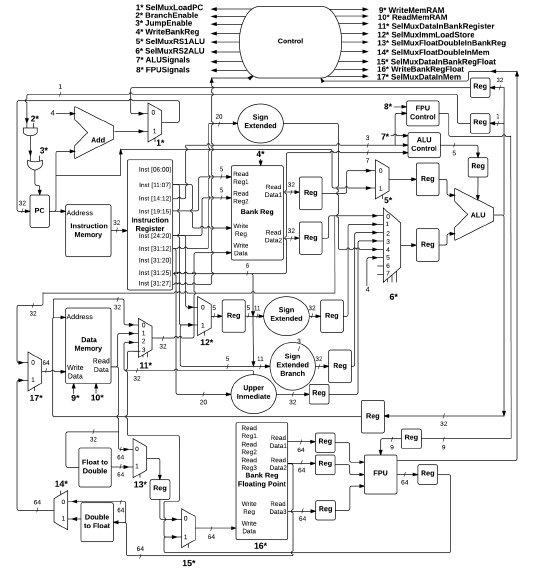
\includegraphics[width=\textwidth]{Micro.jpg}
\centering
\caption{Diagrama funcional del microprocesador ASP. RISC-V. Imágen tomada del trabajo \cite{Carlosthesis}, con la autorización del M.Sc Salazar.}
\label{fig:micro}
\end{figure}

La estructura del RTL de las memorias consiste en desarrollar pequeños bloques de memorias de ocho bits y generar un bloque de memoria total de treinta y dos bits. La técnica de codificación usada corresponde a un arreglo bidimensional en Verilog. En el caso de la memoria de programa o instrucciones, se crea un bloque de memoria de 32 Kbytes (kilo bytes), y se replica cuatro veces para tener una memoria de 32 Kbytes con un tamaño de palabra de treinta y dos bits. Lo mismo debe hacerse con la memoria de datos. 

Sintetizar esta estructura de memorias directamente en la herramienta Design Compiler no es viable pues la misma no está diseñada para sintetizar memorias. Es por ello que conviene incluir bloques de memoria (SRAM en este caso), deben generarse por aparte y luego incluirse como IP Cores dentro del proceso de síntesis física.

Un detalle a considerar es que, al estudiar la estructura del diseño, se descubrió que no se ha generado una estructura en el ASP capaz de inicializar estas memorias (no existe tampoco un esquema adecuado de boot-strap).  Esta situación deberá resolverse en otro proyecto, pero para este trae como consecuencia que no será posible hacer una validación funcional completa del circuito una vez terminado el flujo de implementación. 

Existe una particularidad extra a este proyecto, y consiste en que la unidad de punto flotante original fue desarrollada por el Ing. Diego Rodríguez \cite{Diego2015}; sin embargo, el diseño tenía muchas oportunidades de mejora, por lo que fue optimizada por el Ing. Francis López \cite{Francis2016}. Esta última no fue probada junto al microprocesador, aunque se demostró su funcionabilidad de forma individual. Al igual que con el caso anterior, tampoco será posible hacer una validación de esta etapa pues no ha sido integrada correctamente al ASP. Se procederá con la implementación de la FPU de \cite{Diego2015} simplemente para completar el flujo correcto. Una vez resueltos los problemas de boot-strap, inicialización de memorias e incorporación de la FPU mejorada, será cuestión de corregir brevemente los scripts.

\section{Estrategia de síntesis y validación}

El primer objetivo específico de este trabajo, comprende el someter al ASP a todo el proceso de síntesis lógica. El flujo ya fue expuesto en el capítulo anterior, así que no se entrará en detalles sobre como fue sometido el código, pero se hablará de las configuraciones y consideraciones que se establecieron para que la implementación sea correcta.

\subsection{Restricciones del diseño}
\label{s_sec:const}

Lo expuesto a continuación corresponde a los criterios usados en el scritp de TCL de constraints (restricciones) expuesto en la sección \ref{script_syn}. Este es uno de los puntos de partida fundamentales para la síntesis lógica del ASP.

\subsubsection{Modelo de carga en el cableado (wire\_load\_model)}

El modelo de cableado utilizado en este diseño corresponde al \texttt{ibm13\_wl10} de la biblioteca \texttt{scx3\_cmos8rf\_lpvt\_tt\_1p2v\_25c}. La forma para determinar los modelos de cableado se hace mediante la herramienta Design Compiler y solicitando el reporte de la biblioteca; sin embargo, se debe tener funcionando de forma correcta el Library Compiler. Existen varias modalidades de configuración para el modelo de cableado, en los diseños trabajados en este proyecto se utiliza el modelo ``top".

En el modo superior "top", el compilador de diseño modela las redes como si el diseño no tuviese jerarquía y utiliza el modelo de carga de cable especificado para el nivel superior de la jerarquía de diseño de todas las redes en un diseño y sus subdiseños. La herramienta ignora todos los modelos de carga de cable configurados en subdiseños con el comando \texttt{set\_wire\_load\_model}.

\subsubsection{Reloj y factor de actividad}
\label{subsub:alfa}
Los diseños se diseñan previendo una frecuencia de operación general de 100 MHz por lo que se crea un reloj de con un periodo de 10 ns. Con el fin de modelar un reloj más realista se especifica una transición de 0.5 ns, lo cual se traduce como una pendiente en los flancos de subida y bajada del reloj.

También se específica una incertidumbre con márgenes de setup y de hold de 0.5 ns, que corresponden al lapso entre dos flancos sucesivos respecto a la variación fuera de los tiempos de llegada nominales. Finalmente se especifica una latencia de 0.5 ns, y es básicamente un parámetro que le indica a la herramienta el lapso que se da desde que la señal conmuta en su fuente hasta que conmuta en la entrada de una celda, y su utilidad es sólo para fines de análisis de sincronía y simulación dinámica.

El factor de conmutación ofrece una aproximaxión probabilística al número de veces totales que un circuito conmuta. Así es posible estimar preeliminarmente el consumo dinámico. Este parámetro se configura con una razón de conmutación del 25\% y una probabilidad estática del 50\% pues el reloj es simétrico.

\subsubsection{Puertos y propagación de señales}

Las señales de reloj y reset se configuran para que en ellas se coloquen la mínima cantidad de búfers, y que en general las señales se intervengan de forma mínima en la síntesis. 

Se configura un intervalo de retraso en la propagación de los puertos, con el fin de que los análisis y la simulación sean más realistas, en el caso de las entradas el retardo es 1 ns como mínimo y de 3.5 ns como máximo, y de 1 a 2 ns para las salidas.

Los modelos de la carga asociada a las salidas y entradas se establecen en función de la celda de conducción (\texttt{driving\_cell}), esta configuración le permite a la herramienta de análisis de sincronía estimar de forma precisa el retraso causado desde la conmutación en un puerto, y sobre toda la ruta de propagación consecuente.

Se establece un límite de 10 al máximo fanout para cada celda. El restringir desde la entrada (\texttt{driving\_cell}) hasta la salida (fanout) de cada camino lógico es necesario como punto de partida de las rutinas de optmización de retardo (cálculos de esfuerzo lógico). 

\subsection{Comprobación de la síntesis}
\label{sec:comp_syn}
Como ya se mencionó el diseño de \cite{Carlosthesis}, presenta algunas deficiencias a la hora de considerar someterlo al flujo de diseño digital. En respuesta a lo anterior se efectuó el siguiente proceso.

\begin{enumerate}

\item En primer lugar se modificó el RTL haciendo un \textit{bypass} en la conexión de la memorias, creando puertos para conectar de forma externa las memorias con los módulos que las instanciaban originalmente.

\item Se tomó el RTL original con la FPU diseñado por el Ing. Rodríguez, y se estimuló de acuerdo con el banco de pruebas (\textit{testbench}) proporcionado junto al RTL del ASP. Esta simulación por comportamiento se define como la referencia dorada para validar el diseño.

\item Luego se sustituye la FPU por la diseñada por el Ing. López y se estimula el ASP de nuevo en una simulación por comportamiento para valorar la congruencia con el diseño original.

\item Se sintetiza entonces el RTL sin el banco de memorias.

\item Se realiza una simulación post síntesis lógica del ASP usando un estrategia de simulación hibrida, en el sentido de que se combinan elementos de RTL por comportamiento y post síntesis. Así se pretende modelar las memorias como elementos ideales y poder comprobar la funcionalidad del ASP.
\end{enumerate}

%\section{Resultados de la síntesis lógica del ASP.}

%Habiendo definido el entorno particular en el que se recibió el RTL y las consideraciones que se tomaron para poder comprobar la correcta síntesis del mismo, se muestran los siguientes resultados ofrecidos por los reportes de la herramienta.

%\newpage

%\subsection{Reportes generados en el proceso de síntesis lógica.}
\begin{table}[ht]
\centering
\label{tab:power_asp}
\caption{Resumen del reporte de potencia del microprocesador ASP post síntesis lógica}
\begin{tabular}{||l | c | c | c | c | c |}
\hline
\hline
Group & Internal & Switching  & Leakage & Total & \% Attrs \\
\hline
io\_pad & 0.0000 & 0.0000 & 0.0000 & 0.0000 & 0.00\% \\
\hline
memory & 0.0000 & 0.0000 & 0.0000 & 0.0000 & 0.00\% \\
\hline
black\_box & 0.0000 & 0.0000 & 0.0000 & 0.0000 & 0.00\% \\
\hline
clock\_network & 0.0000 & 0.0000 & 0.0000 & 0.0000 & 0.00\% \\
\hline
register & 7.9920 & 4.2648e-02 & 1.7974e+05 & 8.0349 & 84.01\%\\
\hline
sequential  & 0.0000 & 0.0000 & 0.0000 & 0.0000 & 0.00\% \\
\hline
combinational & 0.1635 & 1.3654 & 3.6572e+05 & 1.5293 & 15.99\% \\
\hline
Total &  8.1556 mW & 1.4081 mW & 545.4596 nW & 9.5642 mW & 100 \%\\
\hline
\hline
\end{tabular}
\end{table}

%\newpage
\begin{lstlisting}[caption={Reporte de área del microprocesador ASP post síntesis lógica.} \label{lst:asp_area_report}, frame={single}]
****************************************
Report : area
Design : MainHMM_2
Version: L-2016.03-SP3
Date   : Wed Dec 14 13:21:38 2016
****************************************

	Library(s) Used: scx3_cmos8rf_lpvt_tt_1p2v_25c

          Number of ports:                          920
          Number of nets:                         40225
          Number of cells:                        37979
          Number of combinational cells:          32684
          Number of sequential cells:              5293
          Number of macros/black boxes:               0
          Number of buf/inv:                       8740
          Number of references:                      40

          Combinational area:             318738.243849
          Buf/Inv area:                    49842.720788
          Noncombinational area:          139687.197126
          Macro/Black Box area:                0.000000
          Net Interconnect area:         4646623.786163

          Total cell area:                458425.440975
          Total area:                    5105049.227139
\end{lstlisting}

\newpage

\begin{lstlisting}[caption={Reporte de sincronía del microprocesador ASP post síntesis lógica.} \label{lst:asp_timing_report}, frame={single},basicstyle=\small]
****************************************
Report : timing -path full -delay max -max_paths 1
Design : MainHMM_2 Version: L-2016.03-SP3
****************************************
		Path Group: clk | Path Type: max
  ---------------------------------------------------------------
  Des/Clust/Port     Wire Load Model       Library
  MainHMM_2          ibm13_wl10     scx3_cmos8rf_lpvt_tt_1p2v_25c
  ---------------------------------------------------------------
  Point					Incr		Path
  clock clk (rise edge)			0.00		0.00
  clock network delay (ideal)		1.00		1.00
  $A/State_reg[3]/CK (DFFQX1TS)		0.00 #		1.00 r
  $A/State_reg[3]/Q (DFFQX1TS)		1.05		2.05 f
  CPUMain/U367/Y (INVX4TS)		0.53		2.59 r
  CPUMain/U2567/Y (INVX4TS)		0.49		3.08 f
  CPUMain/U235/Y (OR3X2TS)		0.68		3.76 f
  CPUMain/U972/Y (CLKINVX3TS)		0.57		4.32 r
  CPUMain/U180/Y (NOR2X1TS)		0.47		4.79 f
  CPUMain/U16337/Y (OAI222X4TS)		0.86		5.65 r
  CPUMain/U147/Y (NOR3BX1TS)		0.49		6.14 r
  CPUMain/U134/Y (BUFX3TS)		0.76		6.90 r
  CPUMain/U5970/Y (NOR2X4TS)		0.51		7.41 f
  CPUMain/U20520/Y (NOR2X2TS)		0.72		8.13 r
  CPUMain/U9888/Y (BUFX3TS)		0.88		9.01 r
  CPUMain/U6270/Y (BUFX3TS)		0.83		9.83 r
  CPUMain/U20522/Y (OAI22X1TS)		0.48		10.31 f
  $B/DataOutput_reg[0]/D (DFFQX1TS)	0.00		10.31 f
  data arrival time					10.31
  clock clk (rise edge)			10.00		10.00
  clock network delay (ideal) 		1.00		11.00
  clock uncertainty           		-0.50		10.50
  $B/DataOutput_reg[0]/CK (DFFQX1TS)	0.00		10.50 r
  library setup time			-0.19		10.31
  data required time					0.31
  ---------------------------------------------------------------
  data required time					10.31
  data arrival time					-10.31
  ---------------------------------------------------------------
  slack (MET)						0.00
  ---------------------------------------------------------------
  Notes:
  	$A = CPUMain/ExtensionFloat.FSMControlCPUFloatPoint
  	$B = CPUMain/BankRegisterInteger/Registro5_t0
\end{lstlisting}

\newpage

%\subsection{Simulaciones}
%\subsubsection{Referencia Dorada}

\begin{figure}[ht]
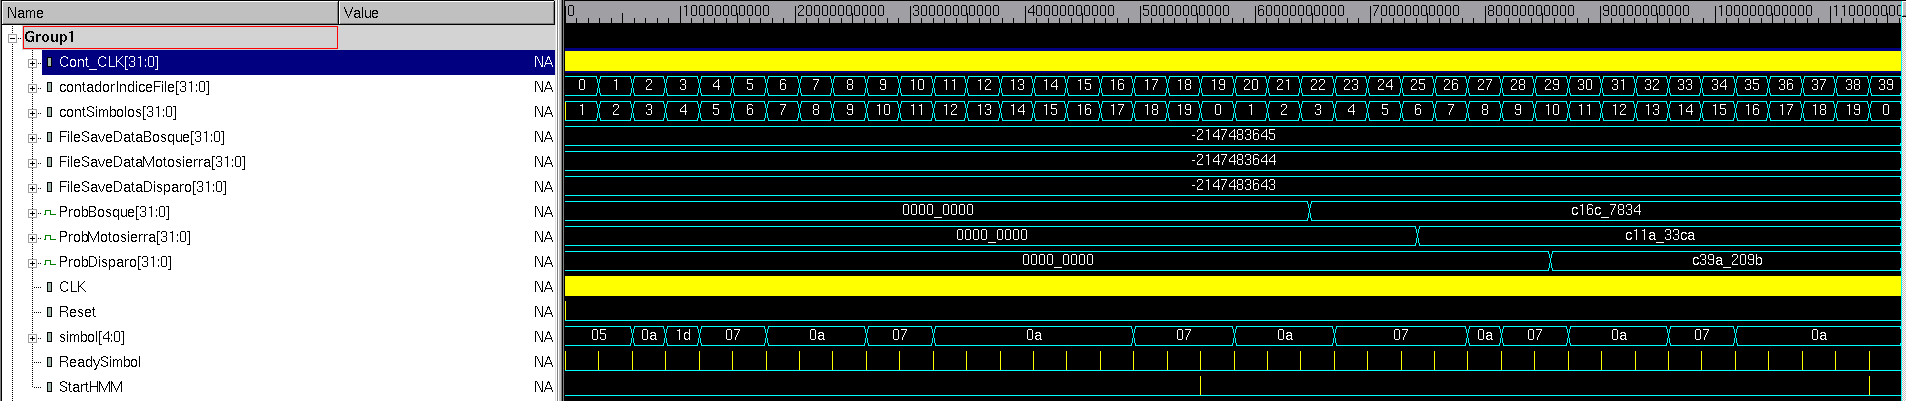
\includegraphics[width=\textwidth]{GR_sim.png}
\centering
\caption{Resultado de la simulación por comportamiento del ASP con la FPU diseñada en \cite{Diego2015}. Según lo estipulado por el M.Sc Salazar en \cite{Carlosthesis}. Esta es la referencia dorada para este trabajo.}
\label{fig:gr_sim}
\end{figure}

\subsubsection{Algoritmo HMM ejecutado en el ASP}
\begin{figure}[h]
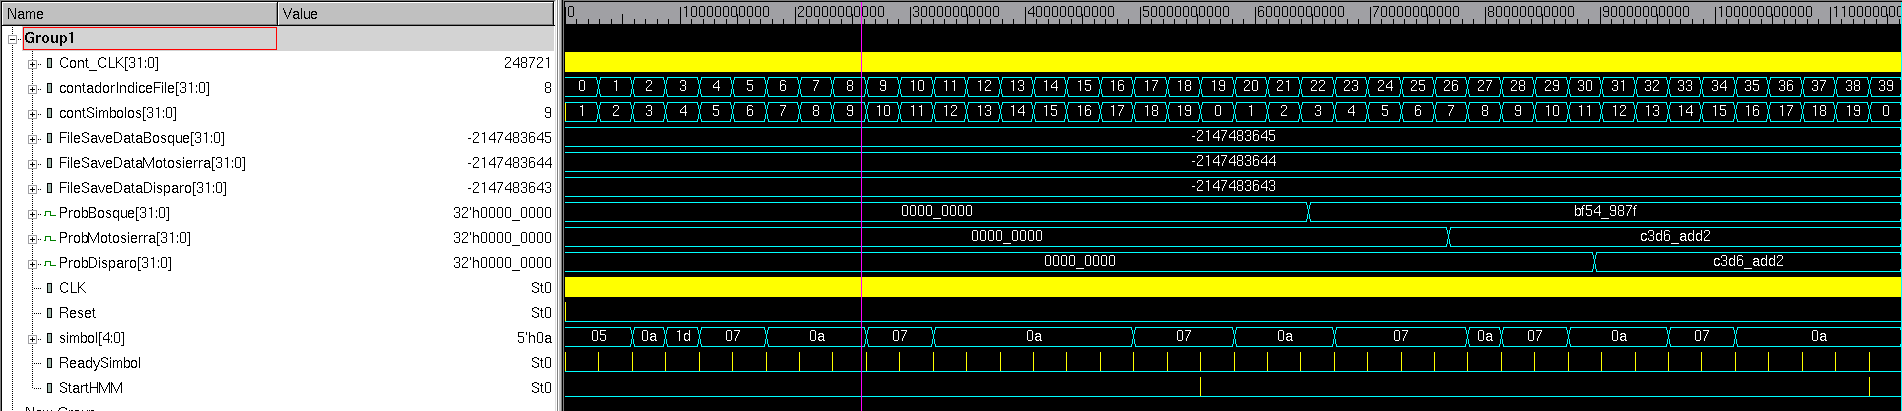
\includegraphics[width=\textwidth]{asp_beh_sim.png}
\centering
\caption{Verificación del funcionamiento del ASP al cambiar la FPU por la versión mejorada de \cite{Francis2016, concapan}. El resultado final del cálculo de probabilidad es erróneo.}
\label{fig:asp_beh_sim}
\end{figure}

\begin{figure}[h]
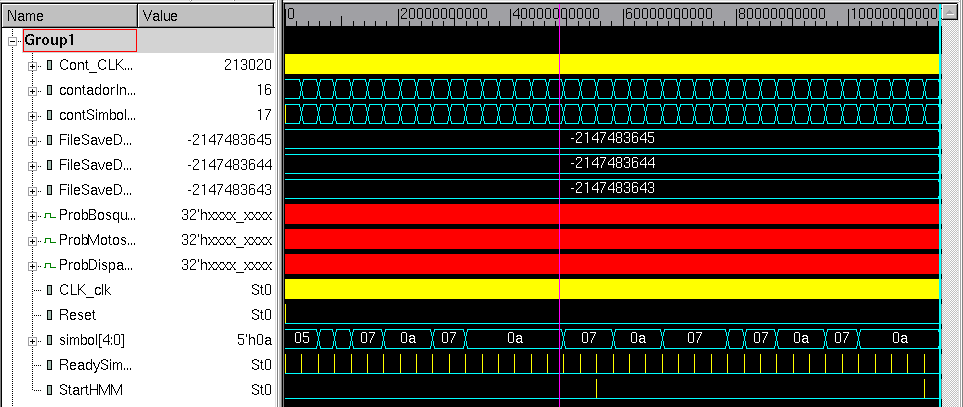
\includegraphics[width=\textwidth]{asp_syn_sim.png}
\centering
\caption{Resultado de simulación post síntesis lógica del ASP, con la FPU de \cite{Francis2016, concapan}. Nótese la existencia de señales indefinidas. Un análisis más detallado mostrará violaciones en la restricción de tiempo de mantenimiento en el resultado de la síntesis lógica.}
\label{fig:asp_syn_sim}
\end{figure}

\begin{figure}[h]
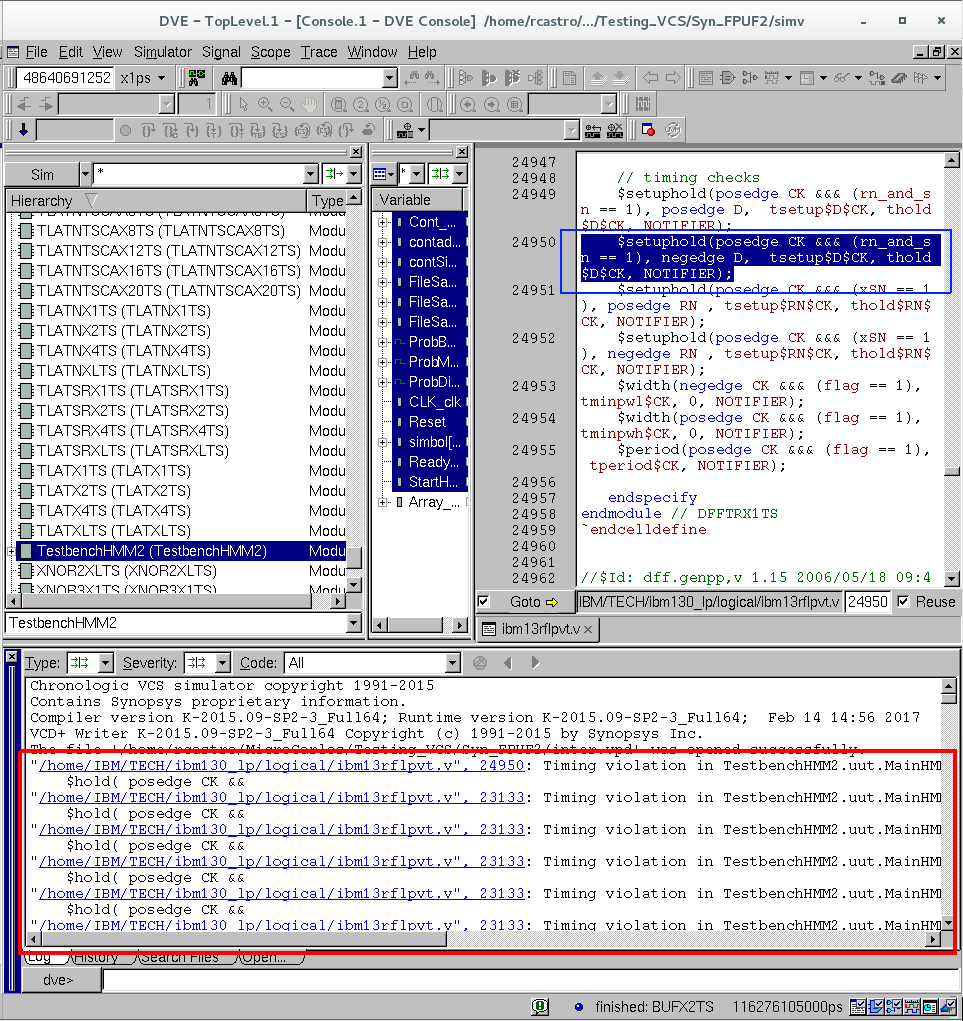
\includegraphics[width=\textwidth]{asp_hold_rape.png}
\caption{Detalle de los resultados de la verificación post-síntesis, proporcionados por VCS. Nóstese la violación de hold. Esto implica que hay que corregir el problema, ya sea desde DesignCompiler, o modificando el RTL si el DC no logra su cometido.}
\label{fig_asp_hold}
\end{figure}

\section{Análisis de resultado: síntesis lógica del ASP}

\subsection{Evaluación pre síntesis}

Se realizó un análisis a nivel de comportamiento del código del ASP que incorpora la FPU desarrollada en \cite{Diego2015}.

Los datos observados en las figuras \ref{fig:gr_sim}, \ref{fig:asp_beh_sim} \ref{fig:asp_syn_sim} correspondientes a los vectores de salida: \texttt{ProbBosque}, \texttt{ProbMotosierra}, y \texttt{ProbDisparo} son datos en hexadecimal, que representan un número en punto flotante de precisión simple, según el estándar IEEE574. Por lo tanto tenemos que para la figura \ref{fig:gr_sim}, según el estímulo usado (definido en el \textit{testbench}, aportado junto al \textit{RTL}) los valores corresponden a -14,779346 para \texttt{ProbBosque}, -9,637644 para \texttt{ProbMotosierra} , y -308,25473 para \texttt{ProbDisparo}.

Según se expone en \cite{Carlosthesis} los valores puntualmente no corresponden a una estadística, pues no existen probabilidades negativas, por lo que estos valores son más una heurística que permite determinar que tan cercano se encuentra un dato a pertenecer a uno de los tres conjuntos mencionados; específicamente, qué tan cercanos se encuentren estos valores a cero. Observando que para la figura \ref{fig:gr_sim}, se aprecia que el valor más cercano a cero (en otras palabras, con una probabilidad más cerca de uno), corresponde al vector \texttt{ProbMotosierra}, por lo tanto, el estímulo tiene una probabilidad más alta de pertenecer a un patrón acústico tipo motosierra; sin embargo, existe una probabilidad modesta de asociar el estímulo al patrón acústico del bosque, lo cual es esperable de acuerdo con las condiciones en las que fueron adquiridos los sonidos que se usaron como estímulos. Finalmente se observa que el estímulo definitivamente no puede considerarse como un disparo, pues su valor se encuentra dos ordenes de magnitud lejos del cero (más detalles del funcionamiento del sistema de clasificador completo puede hallarse en \cite{Carlosthesis, lascas_carlos, concapan}).

Partiendo de la premisa de que el \textit{testbench} contiene un estímulo que corresponde al patrón acústico de una motosierra, se procede a efectuar un contraste entre las figuras \ref{fig:gr_sim}, \ref{fig:asp_beh_sim}. En este se puede encontrar que \texttt{ProbBosque} tiene un valor -0,8304519 (0xbf54987f), mientras que \texttt{ProbMotosierra} y \texttt{ProbDisparo} tienen un valor de -429,35797 (0xc3d6add2). Lo cual según el criterio expuesto anteriormente conduce a considerar que el estímulo es definitivamente sonido de bosque, pues los otros valores están muy lejos del cero. Conociendo que el estímulo en principio es un sonido asociado a una motosierra, y que la respuesta observada en la figura \ref{fig:gr_sim} es correcta, se pudo establecer que la FPU propuesta en \cite{Francis2016} funciona erróneamente. 

\subsection{Evaluación post síntesis}

Ya que el onjetivo de este proyecto es el dejar establecido el flujo de diseño completo, se decidió proseguir con el mismo pese a los errores físicos reportados por las herramientas. Quedará para otro trabajo el corregir los errores en la unidad FPU de \cite{Francis2016}.
%\ref{tab:power_asp}
Como puede observarse en la tabla 4.1, la red de reloj no consume energía, como tampoco los bloques de lógica secuencial. Ello se debe a que al experimentar con el RTL del microprocesador se encontraron las deficiencias la codificación, comentadas anteriormente, por lo que se efectuó la compilación del diseño considerando una red de reloj ideal. Sin embargo, el reporte de potencia permite identificar el grado de consumo de los distintos bloques en el diseño, y dado que se extrajeron los bloques de memoria de este diseño, además de obligar a la herramienta a considerar la red de reloj como una red ideal, puede observarse que el grueso del consumo lo tienen las categorías de registros y lógica combinacional.

El reporte de temporizado, apreciado en el listado \ref{lst:asp_timing_report}, permite observar el comportamiento de la red con el camino crítico, que como ya se mencionó es determinada dinámicamente por la herramienta durante el proceso de compilación en el flujo de la síntesis lógica. Nuevamente el reporte de \textit{timing} permite apreciar que la red de reloj tiene un comportamiento ideal. En este mismo reporte, se ofrece al final una descripción completa de la ruta que sigue la señal más lenta en el diseño. En la primera columna, se va indicando la celda por la que atraviesa la señal (dato) en su camino, la segunda columna indica cuánto retraso aporta a la señal la celda susodicha, y la tercera ofrece un acumulado del retardo hasta ese punto. La suma completa al final de la ruta ofrece el tiempo total de arribo de la señal a su destino (\textit{data arrival time}).

%Falta la ruta de tiempo de llegada del reloj (que en este caso si no se introdujeron estimaciones, debe ser pequeña). El slack es la resta entre el data  expected y el data arrival. tercero indica cuanto retardo se ha acumulado, hasta definir el tiempo que una señal (dato) tarda en propagarse a través del camino crítico (\textit{data arrival time}).

Finalmente en el reporte de timing se consideran los atributos de la red de reloj que se definieron en las restricciones de síntesis, y se define un tiempo límite en el que el dato debería llegar (\textit{data required time}), la diferencia entre el tiempo requerido y el tiempo de arrivo del dato establecen el \textit{slack}, que indica si un diseño funcionaría correctamente a la velocidad requerida. El slack debe ser mayor a cero,  es deseable que ofrezca un margen de seguridad. Un resultado negativo den el slack aquí sería reportado como una violación de setup por la herramienta. No obstante, es conveniente mencionar que, a estas alturas del diseño, estas consideraciones son preliminares (en principio porque puede que la red de reloj no está definida aún de manera muy exacta), y que bien pueden aceptarse violaciones menores en los requerimientos. Es muchas veces posible corregir estas violaciones conforme se traslada el diseño al back end. Por otro lado, una violación significativa (de algunos nanosegundos en relación con los tiempos usados en este diseño), implica un código RTL defectuso que debe corregirse antes de proseguir. Como se puede observar este diseño cumple justamente el \textit{slack}, lo cual es aceptable, aunque suelen ser deseables \textit{slacks} positivos.

Como puede observarse en la simulación post síntesis, las señales correspondientes a los vectores a:
\texttt{ProbBosque, ProbMotosierra, y ProbDisparo}, se encuentran en estado indeterminado (``x"), lo que significa que el modelo de síntesis lógica no está funcionando de la misma manera en que lo hace el RTL; sin embargo, no quiere decir que el producto de la síntesis lógica sea erróneo. Esto quiere decir que la herramienta Design Compiler es capaz de abstraer el diseño de forma correcta en lo que respecta a celdas estándar; la correspondencia entre el comportamiento también depende de las restricciones definidas por el usuario. Al inicio de la sección \ref{subsub:alfa} se definió un factor de transición de 0.5 ns, que implica una pendiente lenta, por lo que el consumo de potencia se eleva, y es muy probable que fallen algunos \textit{flipflos}.

Considerando el escenario de establecido al principio de este capítulo donde se definió que para poder efectuar la síntesis lógica, se iban a extraer los bloques de memoria del microprocesador, y como se planteó posteriormente en la sección \ref{sec:comp_syn}, el proceso de síntesis iba a culminar con una simulación mixta, en el sentido de que se iba a usar el RTL original de los bloques de memorias, junto al GLN generado por la herramienta de síntesis, es de esperar que el diseño no funcione adecuadamente. Una simulación post síntesis trata precisamente de incluir efectos de retardo de las señales. Esta información se obtiene al realizar la síntesis lógica. Un RTL descrito por comportamiento no ofrece información de retardos o temporizado. La herramienta de simulación opera con información incompleta, obteniendo resultados incorrectos.

En la figura \ref{fig_asp_hold} se observa una captura de los mensajes que ofrece la herramienta al compilar la simulación deseada. Como puede apreciarse en la ventana de mensajes, que ha sido resaltada con un recuadro rojo, para este diseño se observa una enorme cantidad de errores de ``hold", es decir que no se cuplen las restricciones físicas de mantemiento (hold) para un registro dado, según indica la herramienta en la ventana de dependencias. En la imagen se resalta uno de los registros en cuestión mediante un recuadro azul. Con esta información es posible buscar los registros ofensores y tratar de hacer cumplir la restricción mediante la inserción manual de retardos en el mismo archivo GLN, o de forma automática, que puede tratar de hacer la misma herramienta con el comando \texttt{set\_fix\_hold}. Esta estrategia fue tomada en cuenta; durante la experimentación con el comando \texttt{set\_fix\_hold} no se logró determinar su uso correcto, y las violaciones de \textit{hold} no fueron corregidas.

Este tipo de errores pueden tener distintas fuentes; sin embargo, el reporte de timing indica que el slack se cumple para el camino crítico, podría analizarse si alguno de los registros ofensores pertenece al camino crítico y realizar las correcciones correpondientes con la herramienta de síntesis. También es posible usar la herramienta para STA y generar un panoráma más amplio sobre que sucede puntualmente con el diseño. Pero partiendo del hecho de que se está realizando una simulación enfocada a un código en GLN, en la que se ha mezclado RTL sin información de retardos y que el diseño se probó erróneo mediante las simulaciones por comportamiento, no es viable intentar optimizarlo.

Finalmente en el listado \ref{lst:asp_area_report} se observa el reporte de área, que es un compendio de la cantidad de elementos y su categoría dentro de la biblioteca, abstrayendo su información en términos de espacio. Este reporte es apenas un estimado de área, pero que sirve al diseñador como punto de partida para cuando deba proponer el plan de piso inicial para su diseño en la etapa de back end. 


